\documentclass[]{paper}
\usepackage{}

% type user-defined commands here
\usepackage{graphicx}
\usepackage{color}
\usepackage{fullpage}
% type user-defined commands here                                                                                                                         
\newif\ifdraft
\drafttrue
\ifdraft
\newcommand{\onote}[1]{ {\textcolor{cyan} { (***Ole: #1) }}}
\newcommand{\terminology}[1]{ {\textcolor{red} {(Terminology used: \textbf{#1}) }}}
\newcommand{\owave}[1]{ {\cyanuwave{#1}}}
\newcommand{\jwave}[1]{ {\reduwave{#1}}}
\newcommand{\alwave}[1]{ {\blueuwave{#1}}}
\newcommand{\jhanote}[1]{ {\textcolor{red} { ***shantenu: #1 }}}
\newcommand{\alnote}[1]{ {\textcolor{green} { ***andreL: #1 }}}
\newcommand{\amnote}[1]{ {\textcolor{blue} { ***andreM: #1 }}}
\newcommand{\smnote}[1]{ {\textcolor{brown} { ***sharath: #1 }}}
\newcommand{\pmnote}[1]{ {\textcolor{brown} { ***Pradeep: #1 }}}
\newcommand{\mrnote}[1]{ {\textcolor{cyan} { ***Melissa: #1 }}}
\newcommand{\note}[1]{ {\textcolor{magenta} { ***Note: #1 }}}
\else
\newcommand{\onote}[1]{}
\newcommand{\terminology}[1]{}
\newcommand{\owave}[1]{#1}
\newcommand{\jwave}[1]{#1}
\newcommand{\alnote}[1]{}
\newcommand{\amnote}[1]{}
\newcommand{\athotanote}[1]{}
\newcommand{\smnote}[1]{}
\newcommand{\pmnote}[1]{}
\newcommand{\jhanote}[1]{}
\newcommand{\mrnote}[1]{}
\newcommand{\note}[1]{}
\fi

\newcommand{\pilotmapreduce}{Pilot-MapReduce\xspace}


\begin{document}

\title{FutureGrid 2012 Project Challenge:\\ Using SAGA to build Scalable Dynamic Distributed Applications}
%\title{FutureGrid 2012 Student Project Challenge} 
\author{Pradeep Kumar Mantha 
  \and Sivakarthik Natesan 
  \and Melissa Romanus 
  \and Sai Saripalli 
  \and Ashley Zebrowski
  \and \large{Faculty Advisor: Shantenu Jha}
}
\date{May 15th, 2012}
\maketitle

\begin{abstract}
\end{abstract}

\section{Introduction}

% The development of scalable and applications presents a formidable research challenge.  

There are multiple challenges in the effective design and implementations of scalable distributed applications and infrastructure: the spectrum of challenges range from managing the heterogeneity inherent in distributed systems on the one hand to the lack of well established programming models to support distributed applications. In addition there do not exist well defined set of base capabilities or unifying abstractions needed to reason about how, when and where to distribute applications. Against this backdrop, the range of distributed cyberinfrastructure (DCI) available to researchers is continually evolving.  Thus, the process of designing and deploying large-scale DCI, as well as developing applications that can effectively utilize them, presents a critical and challenging agenda for domain researchers and CI developers alike.

FutureGrid provides students and researchers with new possibilities to engage in science relating to the state-of-the-art in cloud and grid computing.  As members of the Research in Distributed Cyberinfrastructure and Applications (RADICAL) group, we have taken full advantage of the opportunities that FutureGrid provides.

We have been using SAGA on FutureGrid to address the wide spectrum of challenges: from scalable runtime systems for distributed data-intensive applications (Pilot-MapReduce) to novel dynamic execution modes for traditional HPC applications (Cactus-Spawner) as well as enhanced sampling algorithms (Replica-Exchange).  In addition to flexible and scalable applications, we have used FutureGrid to enhance and extend the capabilities of SAGA.  In this submission we outline how are some of the ways we are using SAGA on FutureGrid resources to push the envelope and pursue exciting new discoveries.

\jhanote{Each section should have the following: Scientific Motivation/objective? How was FutureGrid used? Scientific Results on Futuregrid? Ideally show how this work contributed to Interoperabiltiy and scalability}

\section{Pilot MapReduce}

\jhanote{this needs massive reduction and focus!}

%Scientists in many science disciplines, where enormous amounts of data is generated , e. g. in %the areas of fusion energy, bioinformatics, climate and astronomy, utilize distributed cyber-
%infrastructure to conduct experiments and improve their understanding about the scientific %applications. 

% Scientific Motivation

%Domain scientists face various challenges associated with processing of data at extreme scales, %generated by various data intensive applications on distributed cyberinfrastructures like %FutureGrid. Therefore, an efficient processing of large distributed datasets is required, whilst %deally not introducing fundamentally new programming models or methods. For example, %extending MapReduce - a proven effective programming model for processing large datasets, %to work more effectively on distributed data is desirable. 
%Hadoop is an open-source implementation of MapReduce programming model but is designed %for shared-nothing environments and its performance is affected on a distributed file system.  %On DCI like FutureGrid, we were not able to run Hadoop on multiple clusters due to firewall %issues. MapReduce on distributed data requires effective distributed coordination of %computation (map and reduce) and data, as well as distributed data management (in particular %the transfer of intermediate data units). 

An increasing amount of data that scientific applications need to operate on is distributed. For example, the Earth Science Grid federates data of various climate simulations~\cite{ESG}. Meta-genomic workflows need to process and analyze data generated by various sequencing machines~\cite{Jha:2011fk}; the localization onto a single resource is often not a possibility.
Several options for running Hadoop on distributed data have been proposed~\cite{weissman-mr-11}: (i) in a global Hadoop setup one central JobTracker and HDFS NameNode is used for managing a distributed set of resources; (ii) in a hierarchical Hadoop setup multiple MapReduce clusters are used: a MapReduce cluster close to the data source for pre-processing data and a central cluster for aggregating the different de-central data sources.

Ref~\cite{weissman-mr-11} shows that a hierarchical Hadoop configuration leads to a better performance than a global Hadoop cluster for high data aggregation applications like WordCount. On DCI like FutureGrid, we were not able to run global Hadoop on multiple clusters due to firewall issues.  A drawback of hierarchical Hadoop approach is the increased complexity: Hadoop is not designed with respect to a federation of multiple MapReduce clusters. Setting up such a system typically requires a lot of manual effort.

To address these requirements, we design and implement Pilot-MapReduce (PMR) - a flexible, infrastructure-independent runtime environment for MapReduce. PMR is based on Pilot abstractions for both compute (Pilot-Jobs) and data (Pilot-Data): it utilizes Pilot-Jobs to couple the map phase computation to the nearby source data, and Pilot-Data to move intermediate data using parallel data transfers to the reduce computation phase. Figure ~\ref{fig:mr_arch} depicts the architecture of PMR. 

% PMR Architecture figure.
\begin{figure}[t]
	\centering
	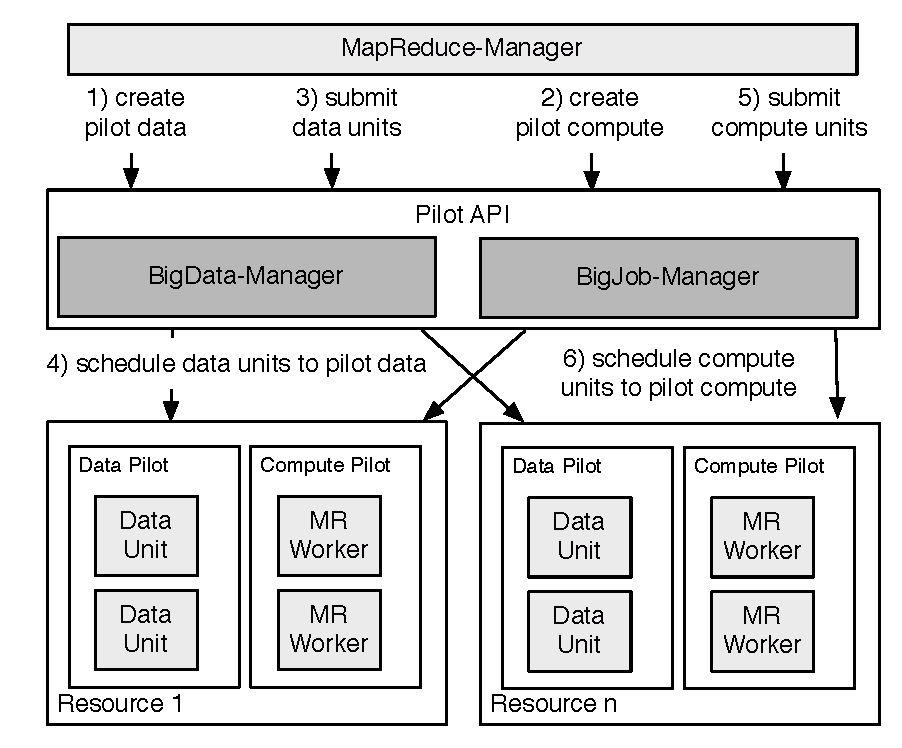
\includegraphics[width=0.38\textwidth]{figures/mr-arch.pdf}
	\caption{\textbf{Pilot-based MapReduce}: Pilot-Jobs manage the map and reduce compute  units and Pilot-data manage the intermediate data transfer between the map and reduce phase across multiple clusters.}
	\label{fig:mr_arch}
\end{figure}

Pilot-MapReduce supports different distributed MapReduce topologies: (i) local, (ii) distributed and (iii) hierarchical. A local PMR performs all map and reduce computations on a single resource. Figure ~\ref{fig:mrtopologies} shows options (ii) and (iii): A distributed PMR utilizes multiple resources often to run map tasks close to the data to avoid costly data transfers; the intermediate data is then moved to another resource for running the reduce tasks. 

%topology picture
\begin{figure}
	\centering
	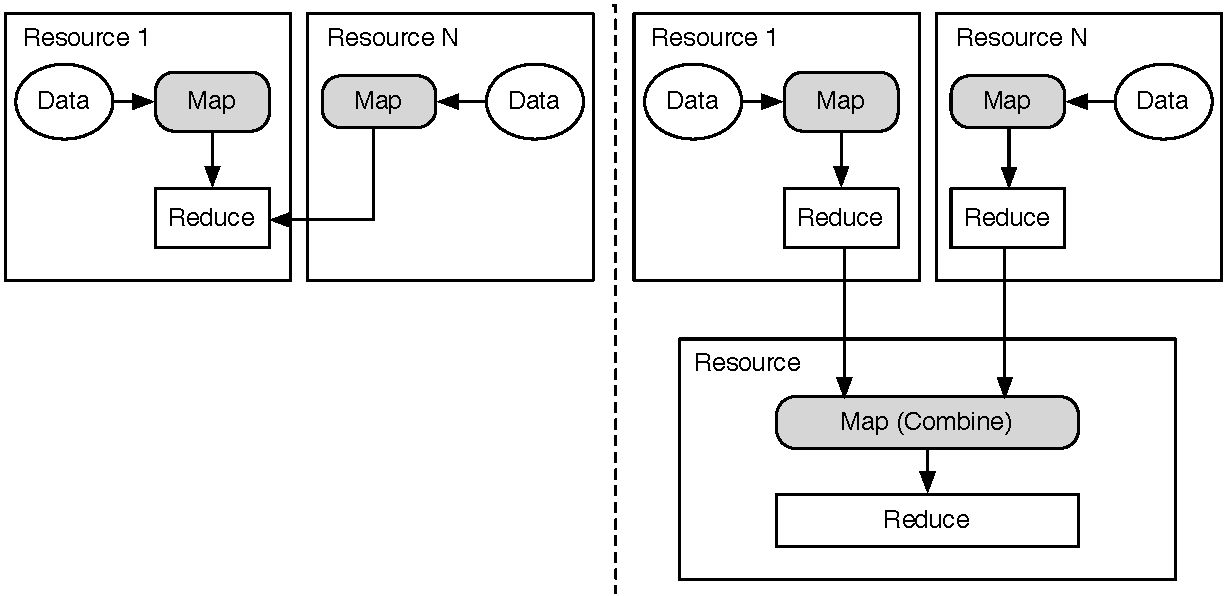
\includegraphics[width=0.42\textwidth]{figures/distributed_hierachical.pdf}
	\caption{\textbf{Pilot-MapReduce Deployment Scenarios}: In the
          distributed scenario (left), the mapping tasks are run close
          to the data; reduced tasks are then run on a single
          resource. In the hierarchical scenario (right) two full
          MapReduce runs are
          conducted. \label{fig:mrtopologies}}
\end{figure}

%%%%%%%%%%%%%%%%%%%
%End Motivation for PMR
%%%%%%%%%%%%%%%%%%%
%How futuregrid is used.
%%%%%%%%%%%%%%%%%%%
FutureGrid has been an important testbed for the development of Pilot abstractions and PMR.
Our experimental evaluations on FutureGrid show that the \textit{innovative} utilization of Pilot abstractions for compute and data treatment in MapReduce framework, across multiple clusters is promising, and can lower the execution time span of the entire MapReduce execution. To demonstrate the performance, extensibility and scalability of PMR, we utilized FutureGrid resources India, Sierra and Hotel.  We benchmarked PMR against Hadoop using various MapReduce topolgoies and each experiment is repeated at least three times.

%Scientific results on futuregrid.
%Performance comparision of Hadoop and PMR on FutureGrid.
In this section we analyze the \textit{performance} and \textit{scalability} of PMR with distributed data and compare it to Hadoop MapReduce using canonical WordCount application on both natural language and random data using different MapReduce topologies.  We utilize two machines, Sierra and Hotel. For all configurations, we use 8 nodes. Table~\ref{tab:data-volumes} summarizes the characteristics of the WordCount application on natural language and random data.

\begin{table}[ht]
	\centering
\begin{tabular}{|p{2cm}|c|c|c|}
\hline
\textbf{Application} &\textbf{Input} &\textbf{Intermediate} &\textbf{Output}\\
%\hline
%GS/PMR 		&80\,GB &71\,GB		 &17\,GB\\
\hline
Word Count\linebreak[4] (English) &16\,GB&26\,GB&20\,MB\\
\hline
Word Count (random) &16\,GB&30\,GB&30\,GB\\
\hline
\end{tabular}
\caption{Data Volumes for different Applications}
\label{tab:data-volumes}
\end{table}

The initial input data of 16\,GB is equally distributed on these two machines. For the single resource
Hadoop configuration, half of the input data needs to be moved from
Sierra to Hotel prior to running the actual MapReduce
job.  Figure~\ref{fig:allmrs_rands} shows the results. For natural language
input, both Hadoop and PMR show comparable performance. A major
determinant of performance for Hadoop (in the case of distributed
data) is the necessity to move parts of the data (half of the input
data) to the central Hadoop cluster. The performance of PMR is
determined by the runtime of the map and reduce phase, which are
slightly longer than for Hadoop mainly due to the resource
heterogeneity and the resulting scheduling overhead: the slowest node
determines the overall runtime of both the map and reduce phase.

Both hierarchical Hadoop and PMR perform better than
the distributed PMR and single resource Hadoop configuration. The
performance is mainly influenced by data movement costs. In the
distributed PMR scenario, half of the {\it intermediate} data needs to
be moved to the other resource; in the hierarchical case half of the
{\it output} data requires movement. Since the output data in the
hierarchical case is a magnitude smaller than the intermediate data in
the distributed case (cmp. table~\ref{tab:data-volumes}) -- 20\,MB in
cmp. to 30\,GB -- the performance in the hierarchical case is
significantly better.

For random data, the distributed PMR and single resource Hadoop
perform better than the hierarchical PMR and hierarchical Hadoop
configuration. As the output data is approximately equal to the
intermediate data (30\,GB), i.\,e.\ the advantage of a reduced
transfer volume does not exit. For random data, the additional
MapReduce run represents an overhead. In the Hadoop case, the moved
data needs to be loaded into HDFS, which represents another overhead.


\begin{figure}[t]
	\centering
		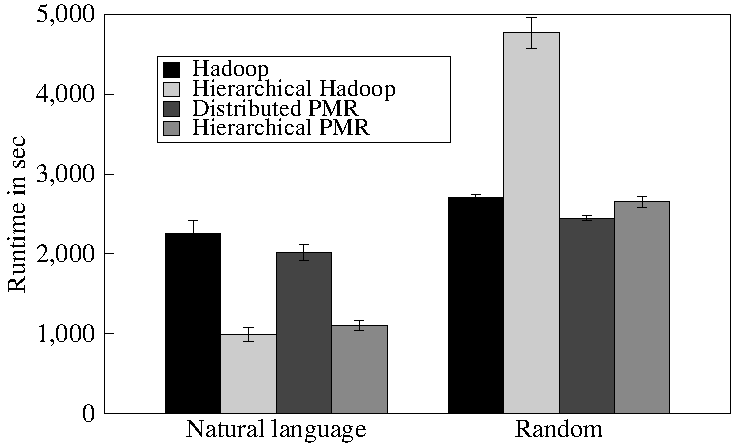
\includegraphics[width=0.47\textwidth]{figures/allmrs_rands.pdf}
\caption{Word Count on 16\,GB Data Using Hadoop, Hierarchical Hadoop, Distributed PMR  and Hierarchical PMR} 	
\label{fig:allmrs_rands}
\end{figure}		

%%%%%%%%%%%%%
%Conclusion
%%%%%%%%%%%%%
%Our experiments show PMR provides the desired flexibility in the deployment and configuration %of MapReduce runs to address specific application characteristics and achieve an optimal %performance, both locally and over wide-area multiple clusters.
Pilot-MapReduce provides a flexible runtime environment for MapReduce applications on general-purpose distributed infrastructures, such as XSEDE and FutureGrid. It brings the advantages of the Pilot abstraction to MapReduce, and enables utilization of federated and heterogeneous compute and data resources. In contrast to Hadoop, no previous cluster setup, which includes running several Hadoop/HDFS daemons, is required. Pilot-MapReduce provides a extensible runtime environment, which allows the flexible usage of sorting in the shuffle, more fine-grained control of data localities and transfer, as well as support for different MapReduce topologies. Using these capabilities, applications with different characteristics, e.g. compute/IO and data aggregation ratios, can be efficiently supported.



\section{Replica Exchange}

Replica-Exchange (RE) methods represent a class of algorithms that involve a large number of loosely-coupled ensembles 
and are used to understand physical phenomena – ranging from protein folding dynamics to binding affinity calculations. The SAGA-based Pilot Framework, BigJob, has been shown to support this class of applications on FutureGrid as well as XSEDE resources.

\mrnote{What do you want to say about this? Abhinav's work?? I am concerned that this overlaps with the fcpc2012-all paper...}



\section{Cactus Spawner - Ashley Zebrowski}
The Cactus Spawner project envisions application frameworks with simulations that
can be broken down to their constituent components and run across multiple
distributed systems.  A chief consideration is that of ``intelligent computing'',
of knowing when and where to run simulation components separately from the main
simulation.  Work is being done to enable this by modelling simulation components
and predicting the time to run locally vs. the time to transport them and execute
them remotely.  To model real-world problems, the Cactus framework is used, and
actual black hole simulations are executed and spawned from.  Contributions
to the field involve algorithms in modelling, spawning, and performance evaluation on
the I/O systems of FutureGrid hardware.

\section{Bliss Development - Ashley Zebrowski}
SSH adaptor, Eucalyptus adaptor enable cloud interoperability.  Working on 
Bliss itself lowers the barrier of entry to distributed computing for developers
of both Bliss-enabled software and Bliss plugins/extensions.

\section{CSA Deployment and Testing}

SAGA and BigJob are deployed on all major FutureGrid machines (India, Sierra, Hotel and Alamo). While it is possible to install and use SAGA and BigJob each user's directory, it would not be without a non-trivial amount of effort in configuration and maintenance. Furthermore, having a central location on each machine where SAGA is deployed as a community code saves time and effort in maintaining the installation and supporting its users. FutureGrid continues providing Community Software Areas (CSA) to communities, which basically is a system level area where software packages can be shared among a community of users. Therefore it was only logical to deploy SAGA and BigJob in a CSA space on FutureGrid machines.

The source code for SAGA and BigJob is stored in a git repository (\cite{bigjob_web}). A github wiki is used to store user guides for each of the individual FutureGrid machines. A BigJob CSA release is the result of a production pipeline. Any newly developed features, code modifications and bug fixes are created in branches and later merged onto the master. Once merged a set of semi-automatic deployment scripts is used to manually trigger the update. The update can encompass an individual machine or all machines, an individual SAGA component or the entire SAGA/BigJob installation. The set of supported components includes the SAGA core libraries, different API packages, the supported middleware adaptors for each machine, the python bindings, and the BigJob package and its dependencies. 

After each update, a set of automated unit tests is run on the target machines to ensure that not only the updated version is deployed, but more importantly, that it is correctly installed and configured for that target machine. The unit tests range from basic (low-level) environment testing, to application level test runs of a BigJob application. The user can also submit own scripts to test the deployments on CSA space. The test README, module file and test results are all committed to the central SAGA code repository, and (partially) used to document the current state of deployment on the SAGA deployment wiki. 


After testing is complete, the python code is pushed to the Python Package Index (\textit{pypi}). This code is then deployed into the CSA space using pypi. Careful consideration is taken to ensure that the updates to CSA space will not impact any current users of BigJob on the XSEDE resources. Another round of testing is then completed to verify that the CSA installations are working and no changes to the users' environments are required. Any corresponding documentation on the github wiki is updated to reflect the changes.


\section{Conclusion}
Here we will evaluate each application based on how they fit into the FutureGrid proposal
criteria.
\begin{enumerate}
\item Interoperability
\item Scalability
\item Contribution to Education
\item Research (innovation, quality of papers, new software, algorithms, insightful performance measurements, etc.)

\end{enumerate}
\begin{thebibliography}{9}
\end{thebibliography}



\end{document}
